\section{Non signal testing of the regular and variational Autoencoder}

\subsection*{Channel removing}
\subsubsection*{Autoencoder}
Both the large and small autoencoder produced results, and are shown below. The small autoencoder results will always be first for each of the tests. 


\begin{figure}[h!]
    \centering
    \begin{subfigure}{.45\textwidth}
        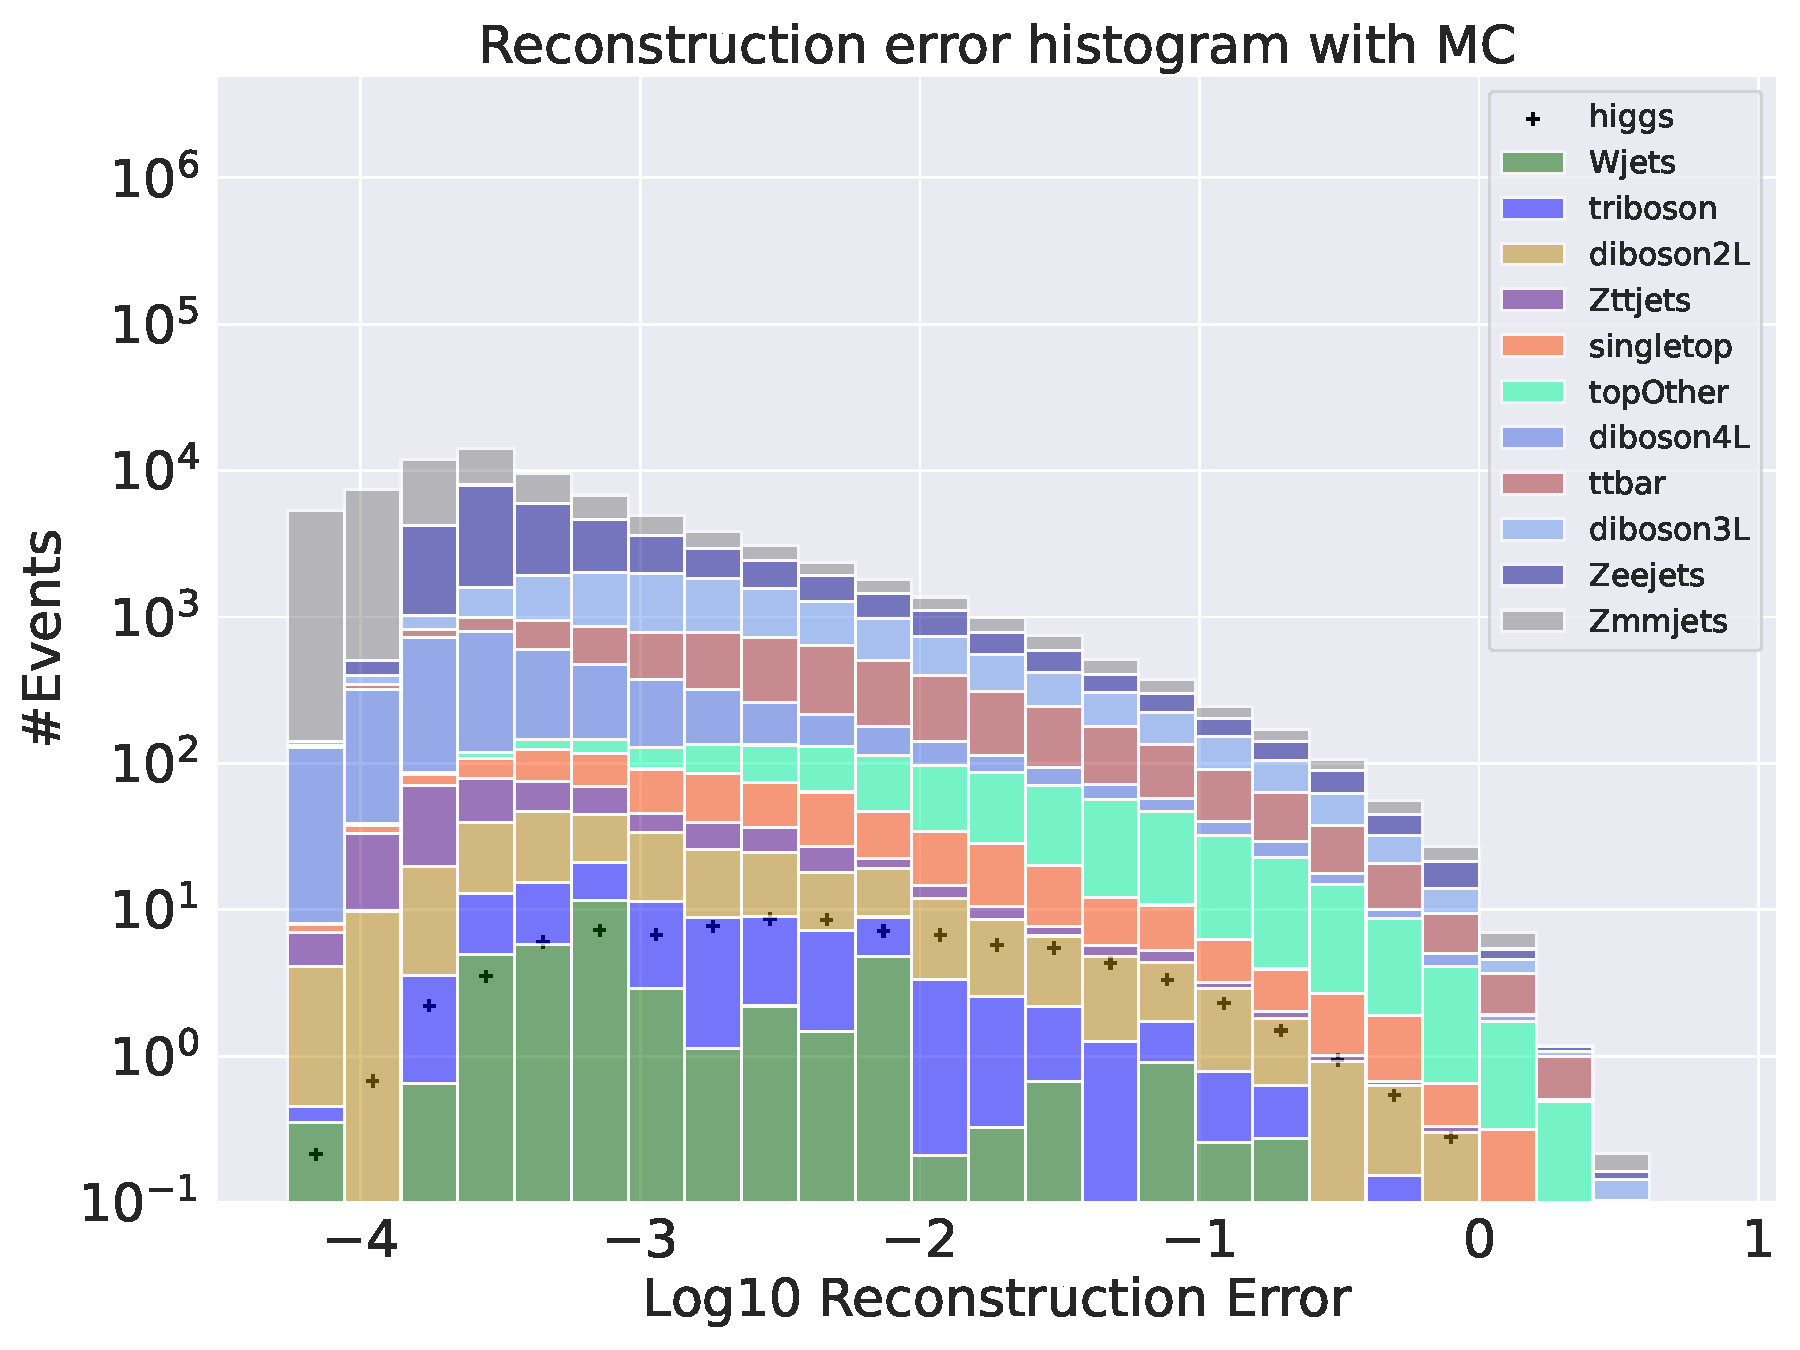
\includegraphics[width=\textwidth]{Figures/AE_testing/small/b_data_recon_big_rm3_feats_sig_higgs.pdf}
        \caption{Reconstruction error on validation SM MC from the small Autoencoder. Here the higgs channel has been removed from training and 
        is used as signal. No significant difference in distributions are found.}
        \label{fig:ae_small_higgs}
    \end{subfigure}
    \hfill 
    \begin{subfigure}{.45\textwidth}
        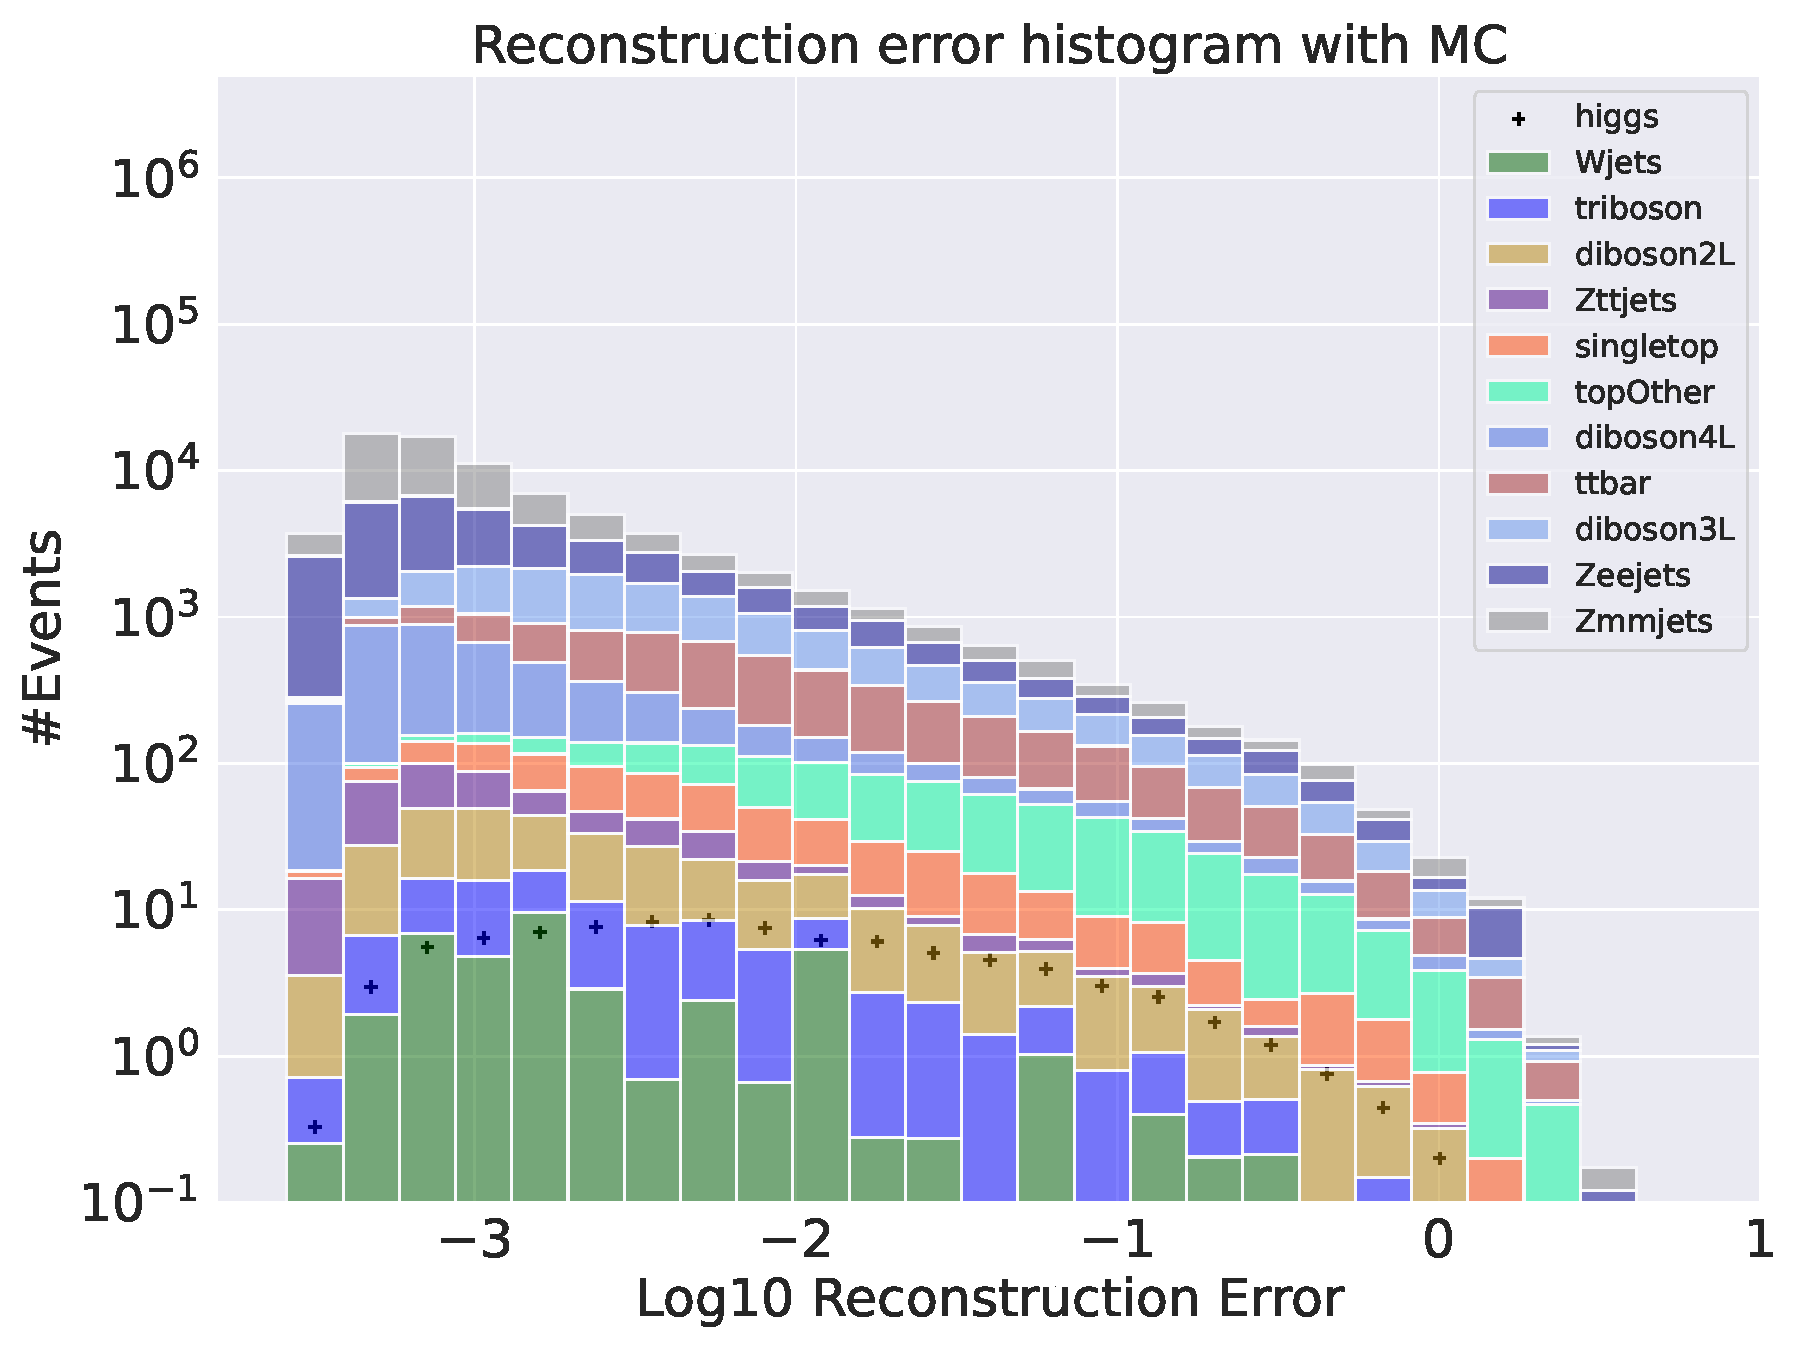
\includegraphics[width=\textwidth]{Figures/AE_testing/big/b_data_recon_big_rm3_feats_sig_higgs.pdf}
        \caption{Reconstruction error on validation SM MC from the big Autoencoder. Here the higgs channel has been removed from training and 
        is used as signal. No significant difference in distributions are found. }
        \label{fig:ae_big_higgs}
    \end{subfigure}
    \hfill  
    \label{fig:ae_big_channel_1}
\end{figure}

\begin{figure}[h!]
    \centering
    \begin{subfigure}{.45\textwidth}
        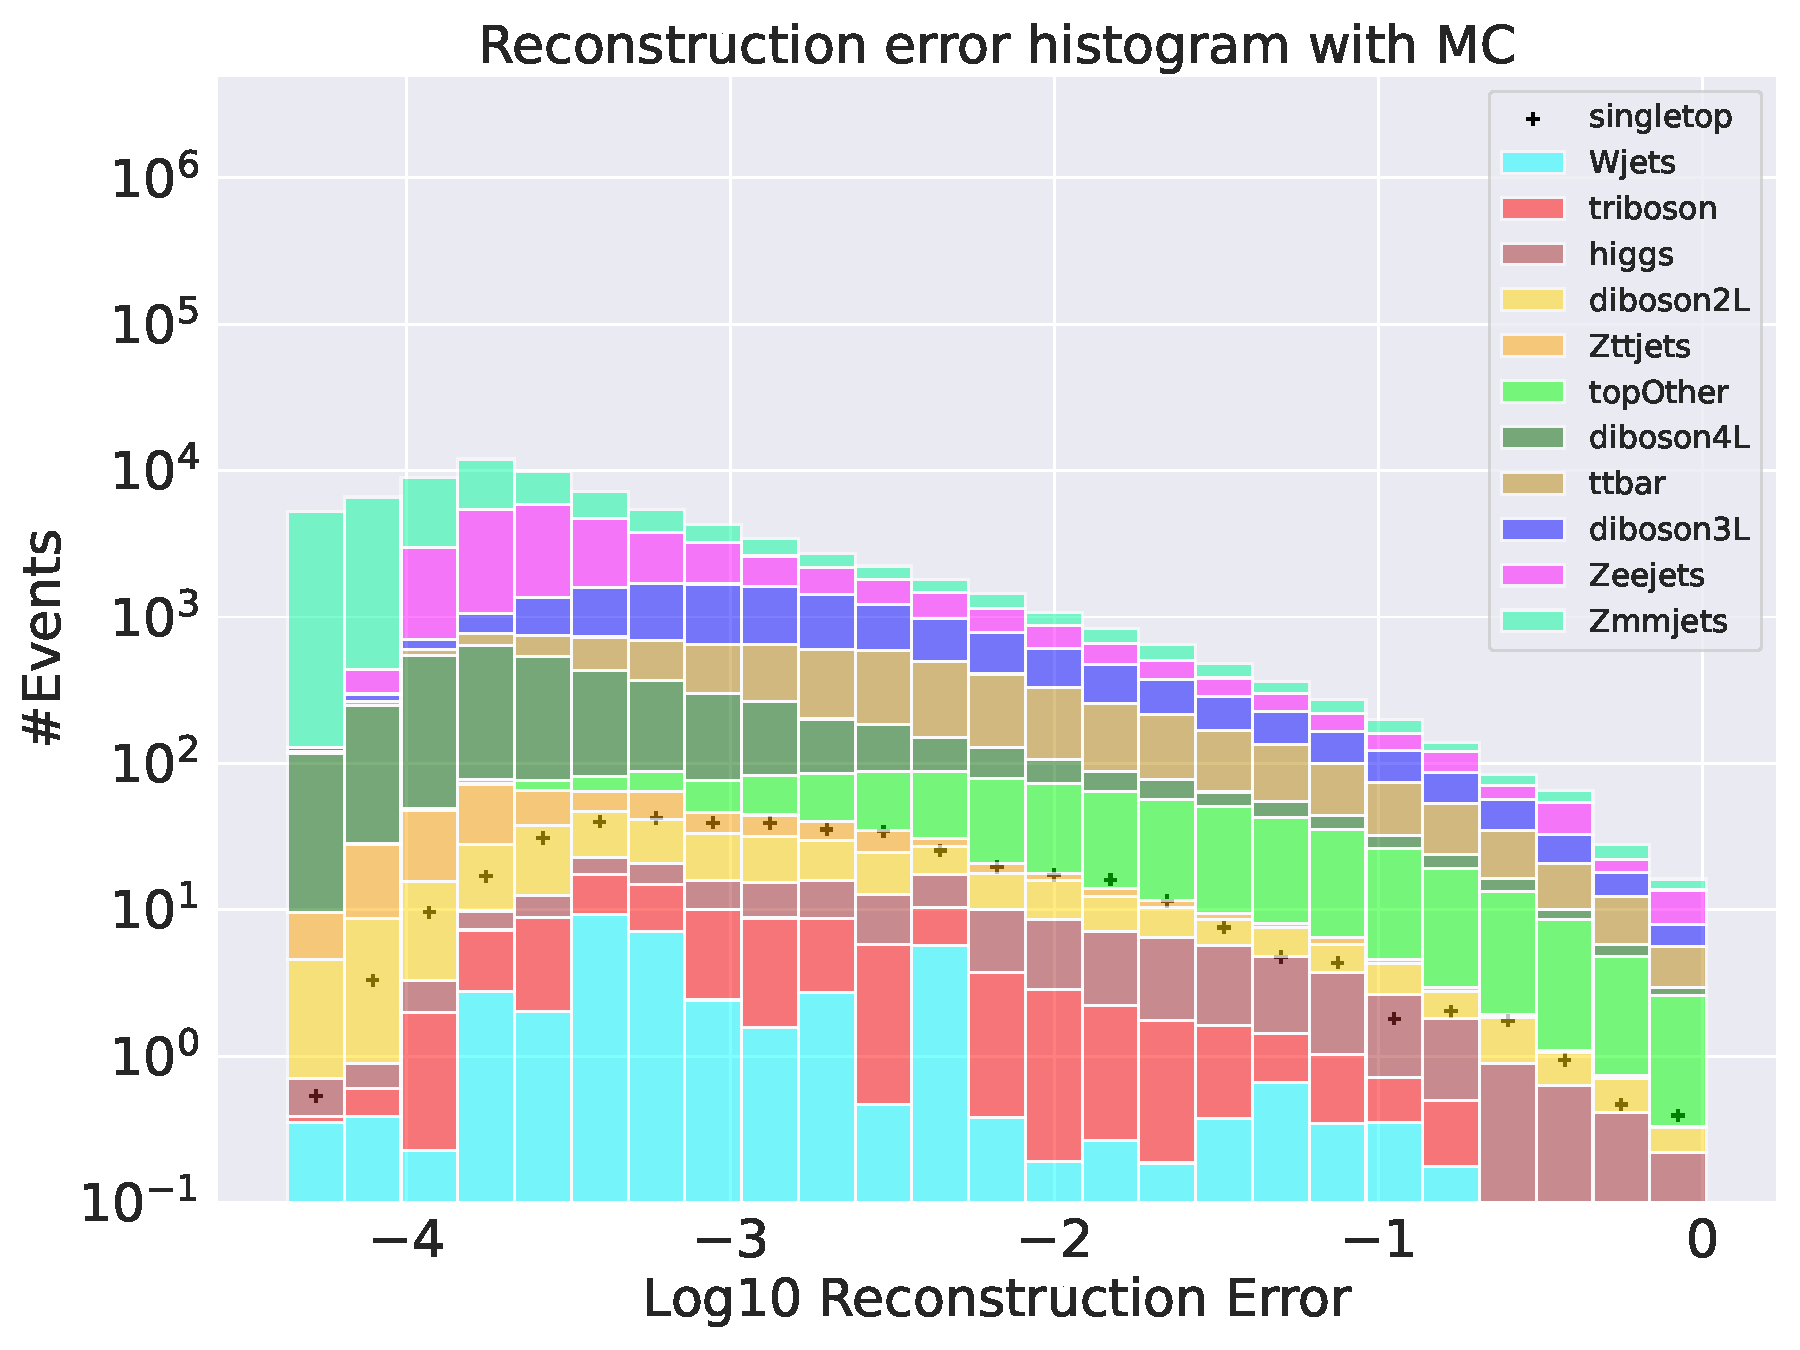
\includegraphics[width=\textwidth]{Figures/AE_testing/small/b_data_recon_big_rm3_feats_sig_singletop.pdf}
        \caption{Reconstruction error on validation SM MC from the small Autoencoder. Here the singletop channel has been removed from training and 
        is used as signal. No significant difference in distributions are found. }
        \label{fig:ae_small_singletop}
    \end{subfigure}
    \hfill
    \begin{subfigure}{.45\textwidth}
        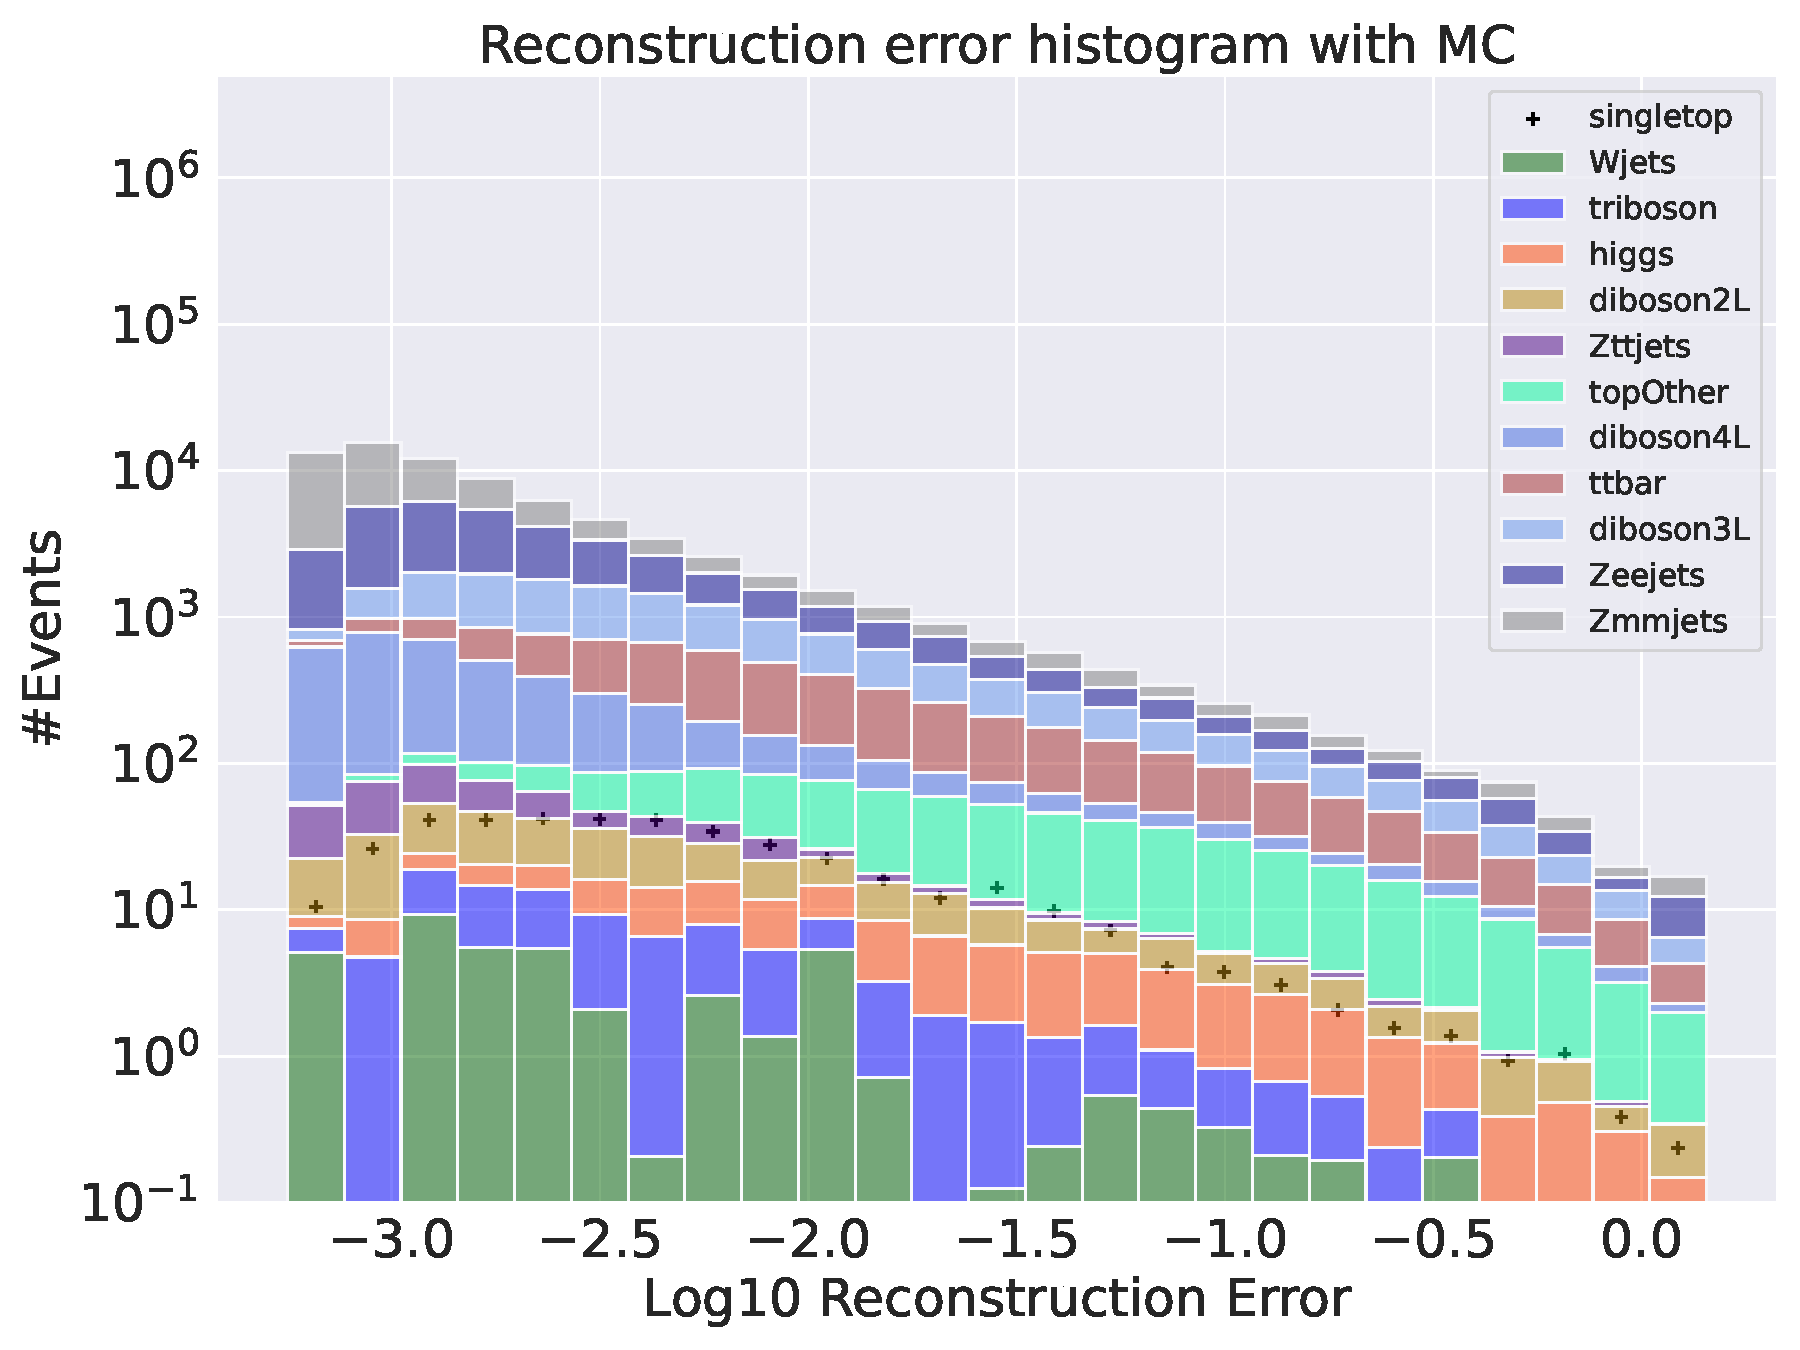
\includegraphics[width=\textwidth]{Figures/AE_testing/big/b_data_recon_big_rm3_feats_sig_singletop.pdf}
        \caption{Reconstruction error on validation SM MC from the big Autoencoder. Here the singletop channel has been removed from training and 
        is used as signal. No significant difference in distributions are found. }
        \label{fig:ae_big_singletop}
    \end{subfigure}
    \hfill 
    \label{fig:ae_big_channel_2}
\end{figure}

\begin{figure}[h!]
    \centering
    \begin{subfigure}{.45\textwidth}
        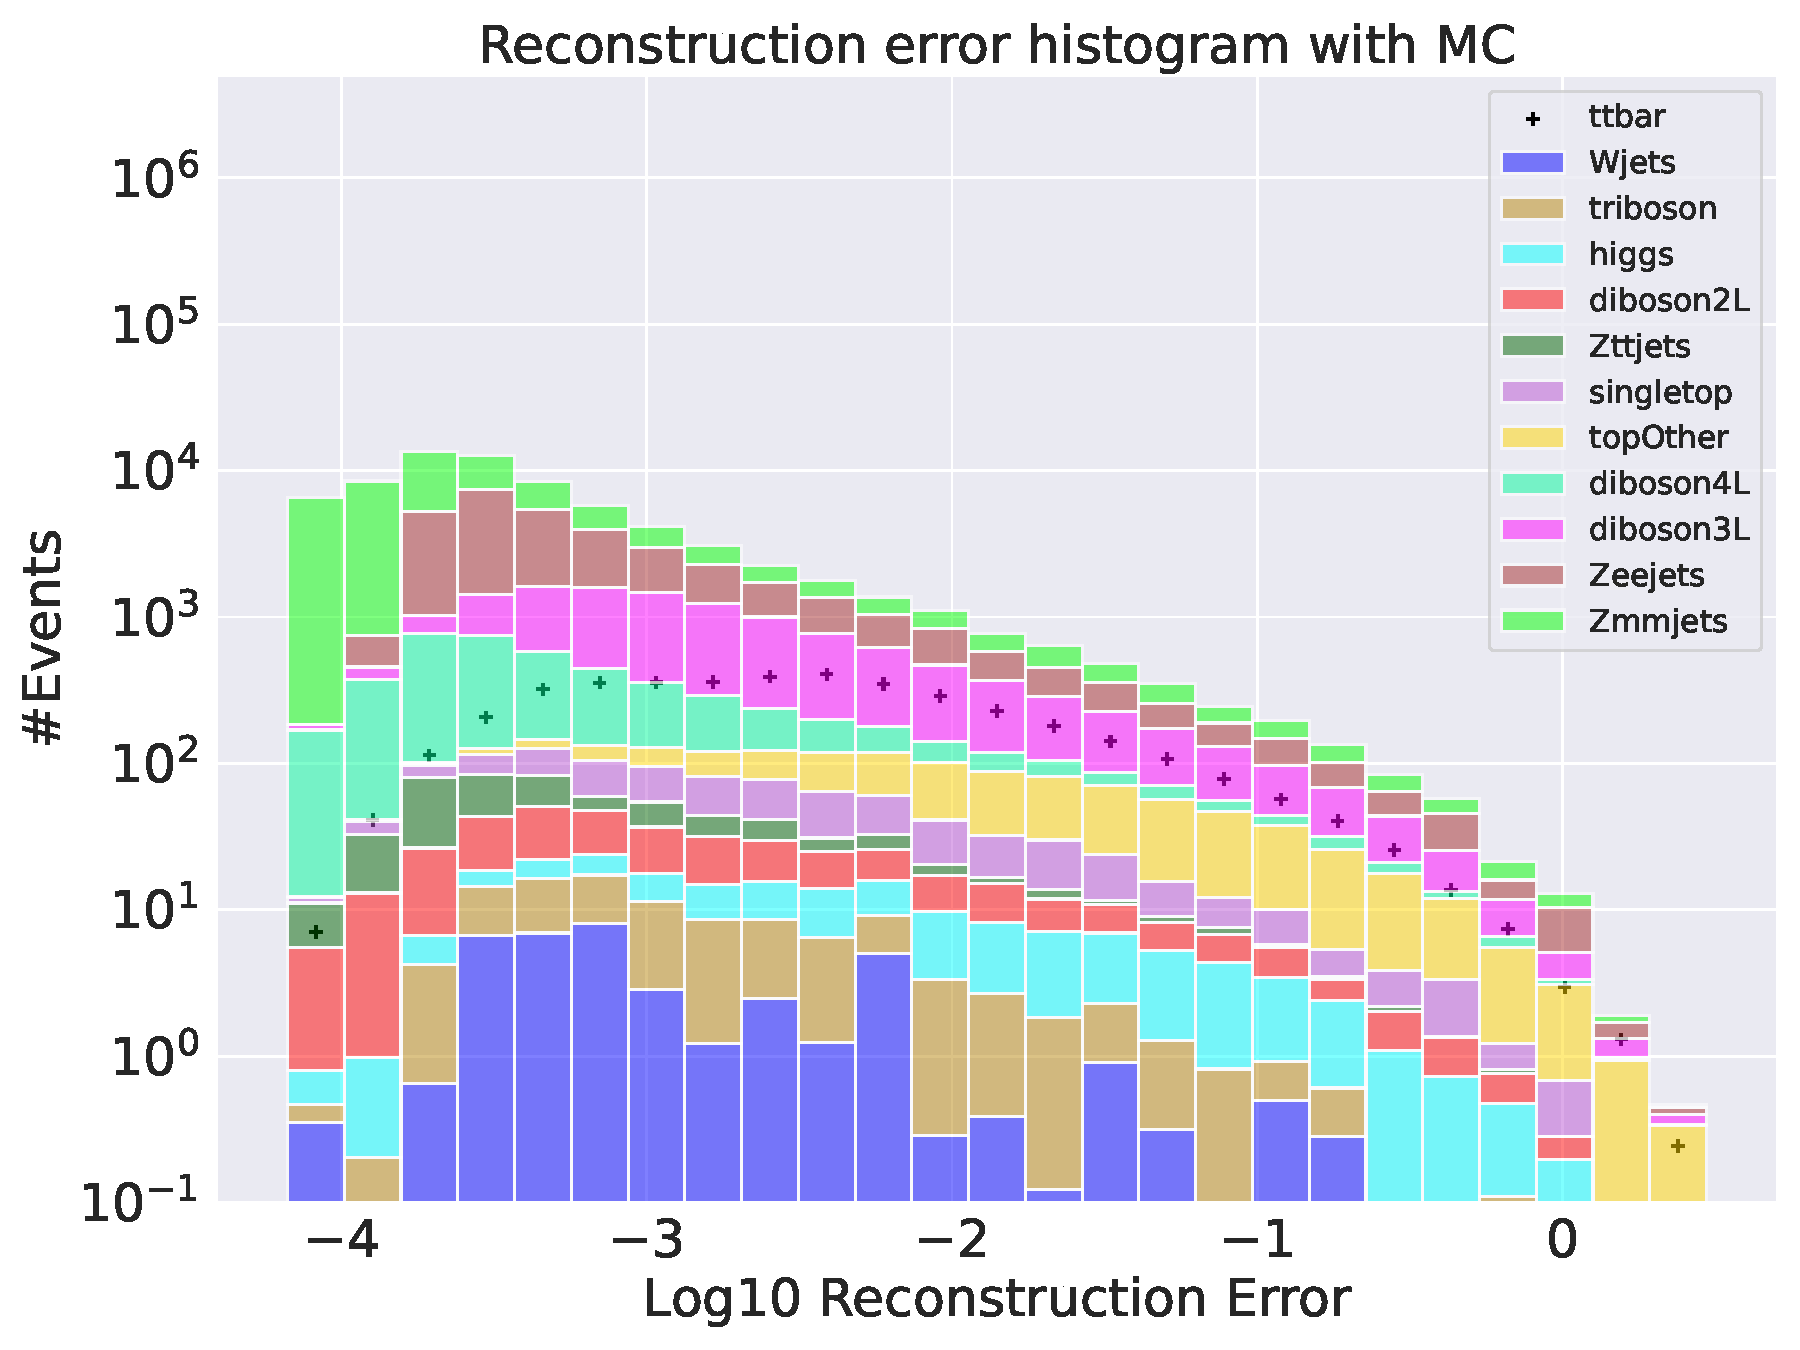
\includegraphics[width=\textwidth]{Figures/AE_testing/small/b_data_recon_big_rm3_feats_sig_ttbar.pdf}
        \caption{Reconstruction error on validation SM MC from the small Autoencoder. Here the ttbar channel has been removed from training and 
        is used as signal. No significant difference in distributions are found. }
        \label{fig:ae_small_ttbar}
    \end{subfigure}
    \hfill 
    \begin{subfigure}{.45\textwidth}
        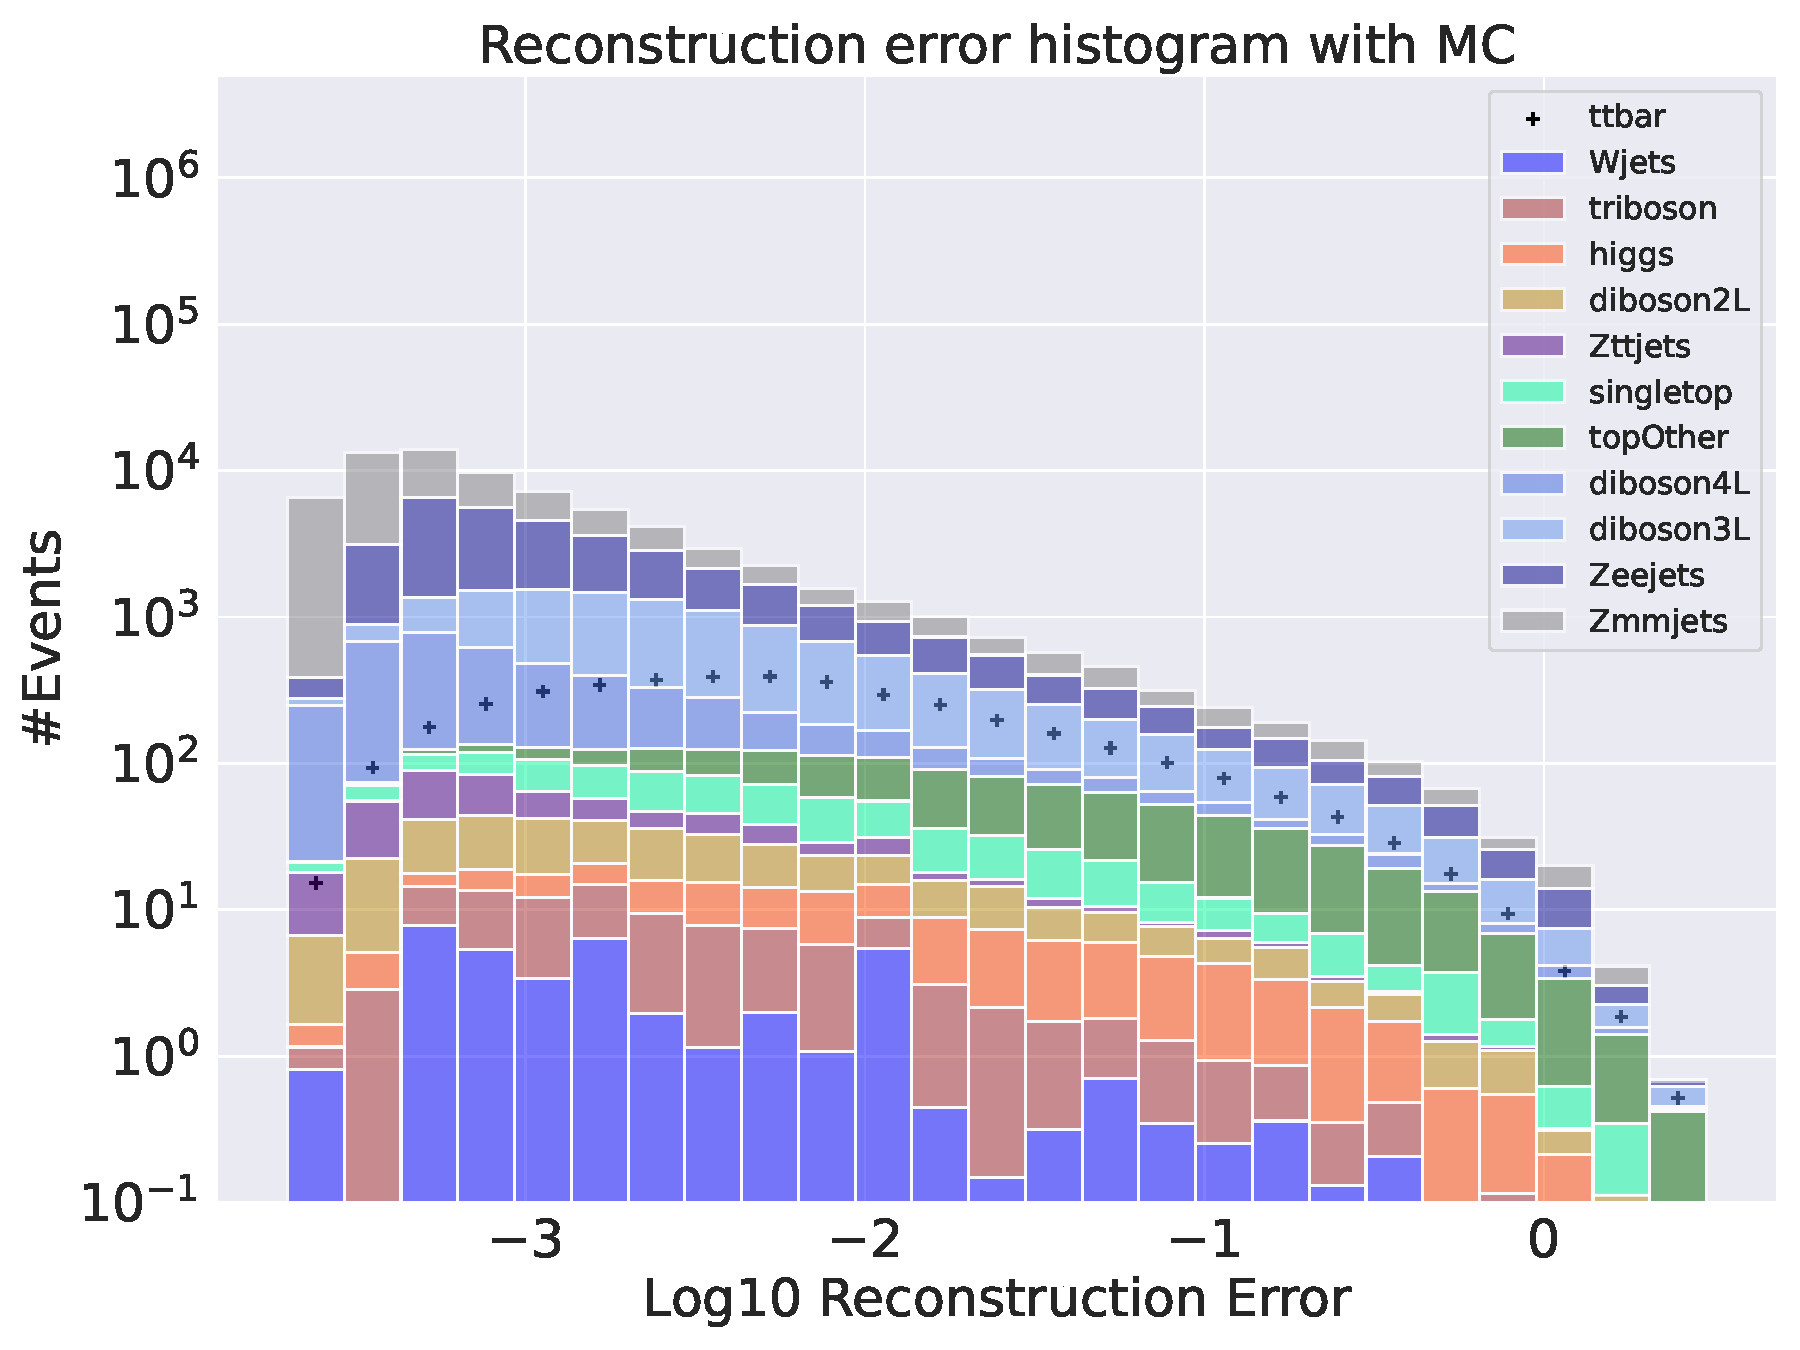
\includegraphics[width=\textwidth]{Figures/AE_testing/big/b_data_recon_big_rm3_feats_sig_ttbar.pdf}
        \caption{Reconstruction error on validation SM MC from the big Autoencoder. Here the ttbar channel has been removed from training and 
        is used as signal. No significant difference in distributions are found. }
        \label{fig:ae_big_ttbar}
    \end{subfigure}
    \hfill 
    \label{fig:ae_big_channel_3}
\end{figure}



\subsubsection*{Variational Autoencoder}
Both the large and small autoencoder produced results, and are shown below. The small autoencoder results will always be first for each of the tests. 


\begin{figure}[h!]
    \centering
    \begin{subfigure}{.45\textwidth}
        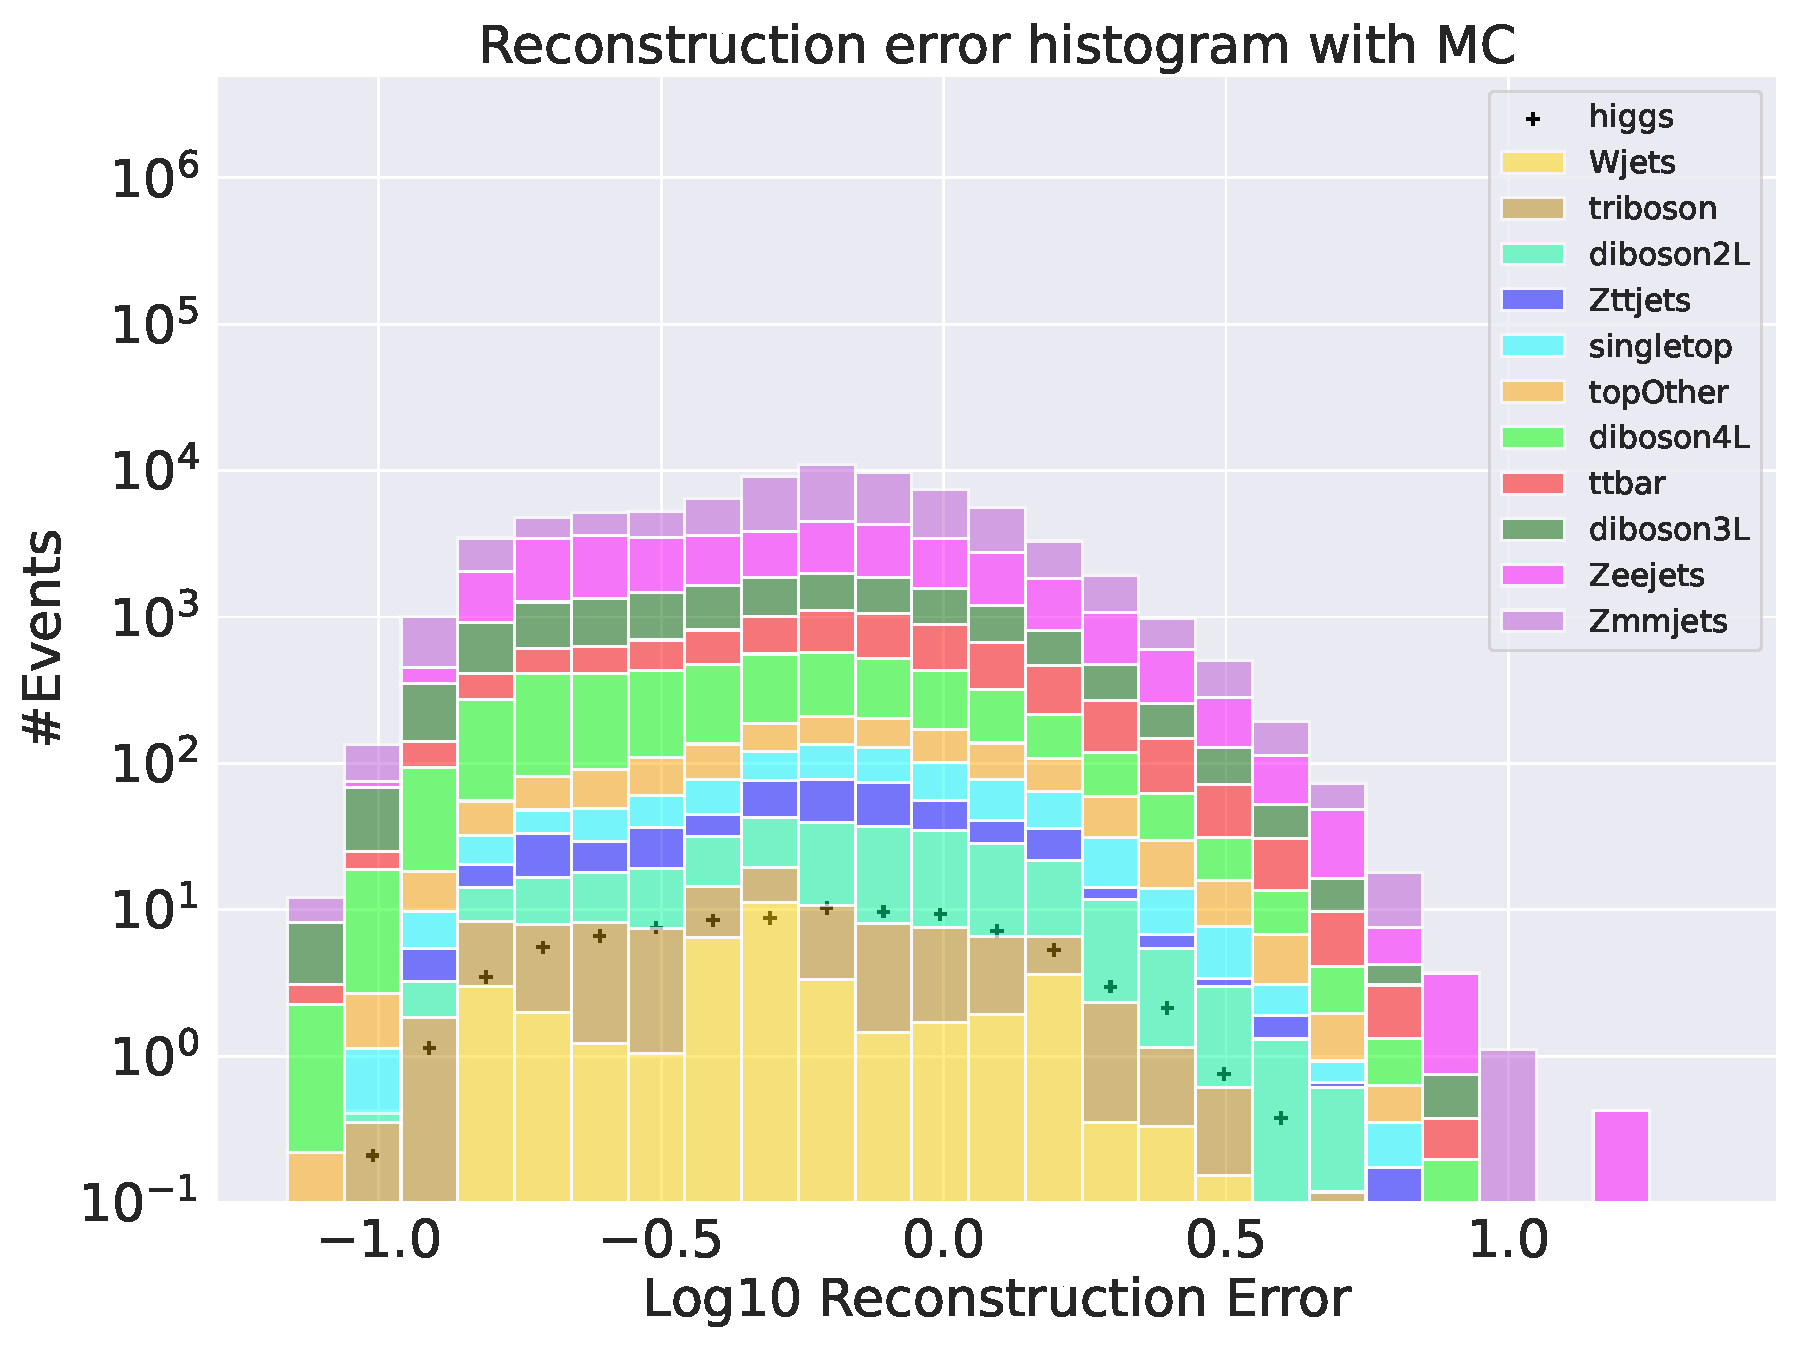
\includegraphics[width=\textwidth]{Figures/VAE_testing/small/b_data_recon_big_rm3_feats_sig_higgs.pdf}
        \caption{Reconstruction error on validation SM MC from the small variational Autoencoder. Here the higgs channel has been removed from training and 
        is used as signal. No significant difference in distributions are found.}
        \label{fig:vae_small_higgs}
    \end{subfigure}
    \hfill 
    \begin{subfigure}{.45\textwidth}
        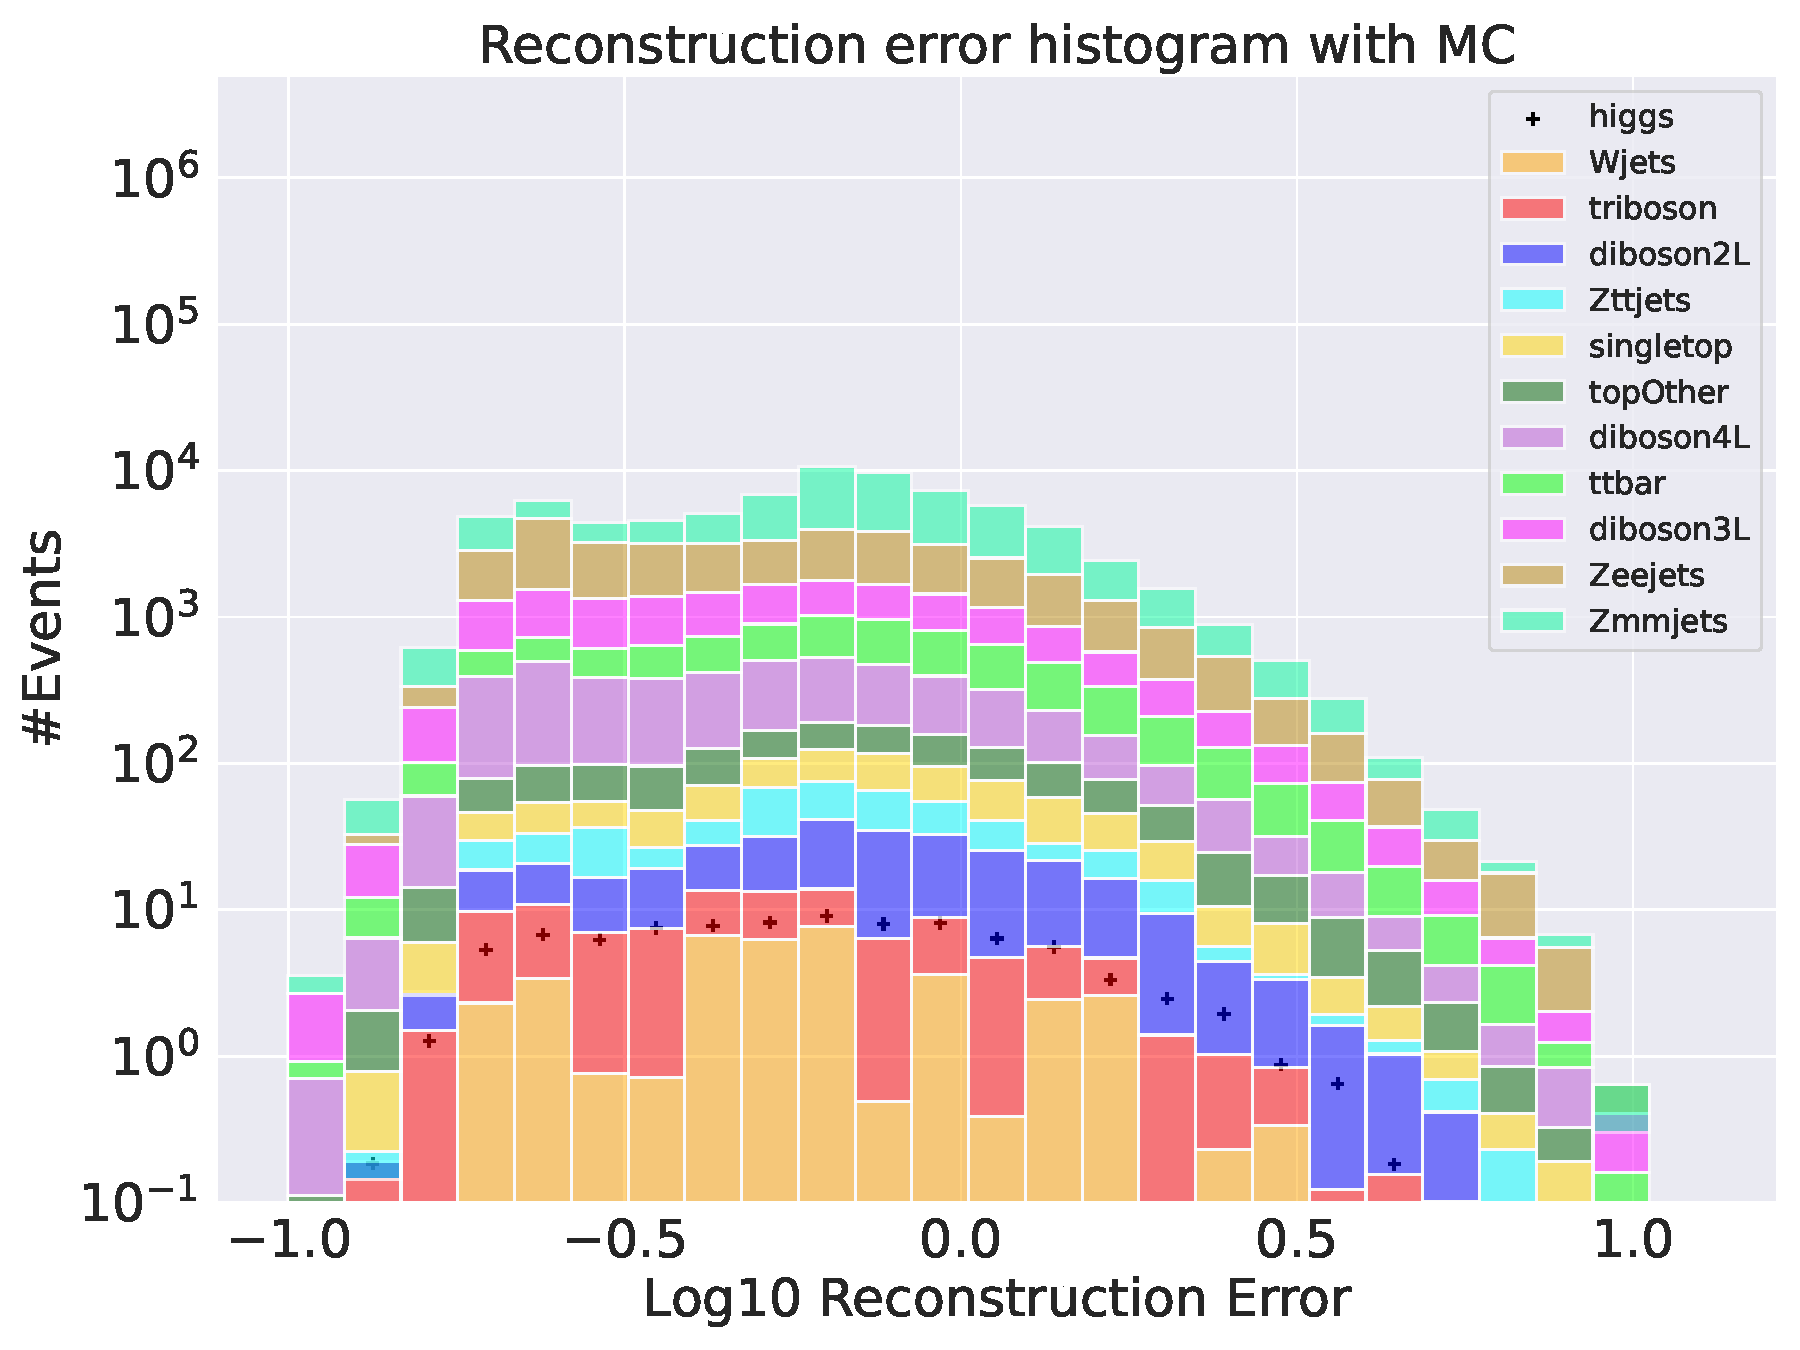
\includegraphics[width=\textwidth]{Figures/VAE_testing/big/b_data_recon_big_rm3_feats_sig_higgs.pdf}
        \caption{Reconstruction error on validation SM MC from the big variational Autoencoder. Here the higgs channel has been removed from training and 
        is used as signal. No significant difference in distributions are found. }
        \label{fig:vae_big_higgs}
    \end{subfigure}
    \hfill  
    \label{fig:vae_big_channel_1}
\end{figure}

\begin{figure}[h!]
    \centering
    \begin{subfigure}{.45\textwidth}
        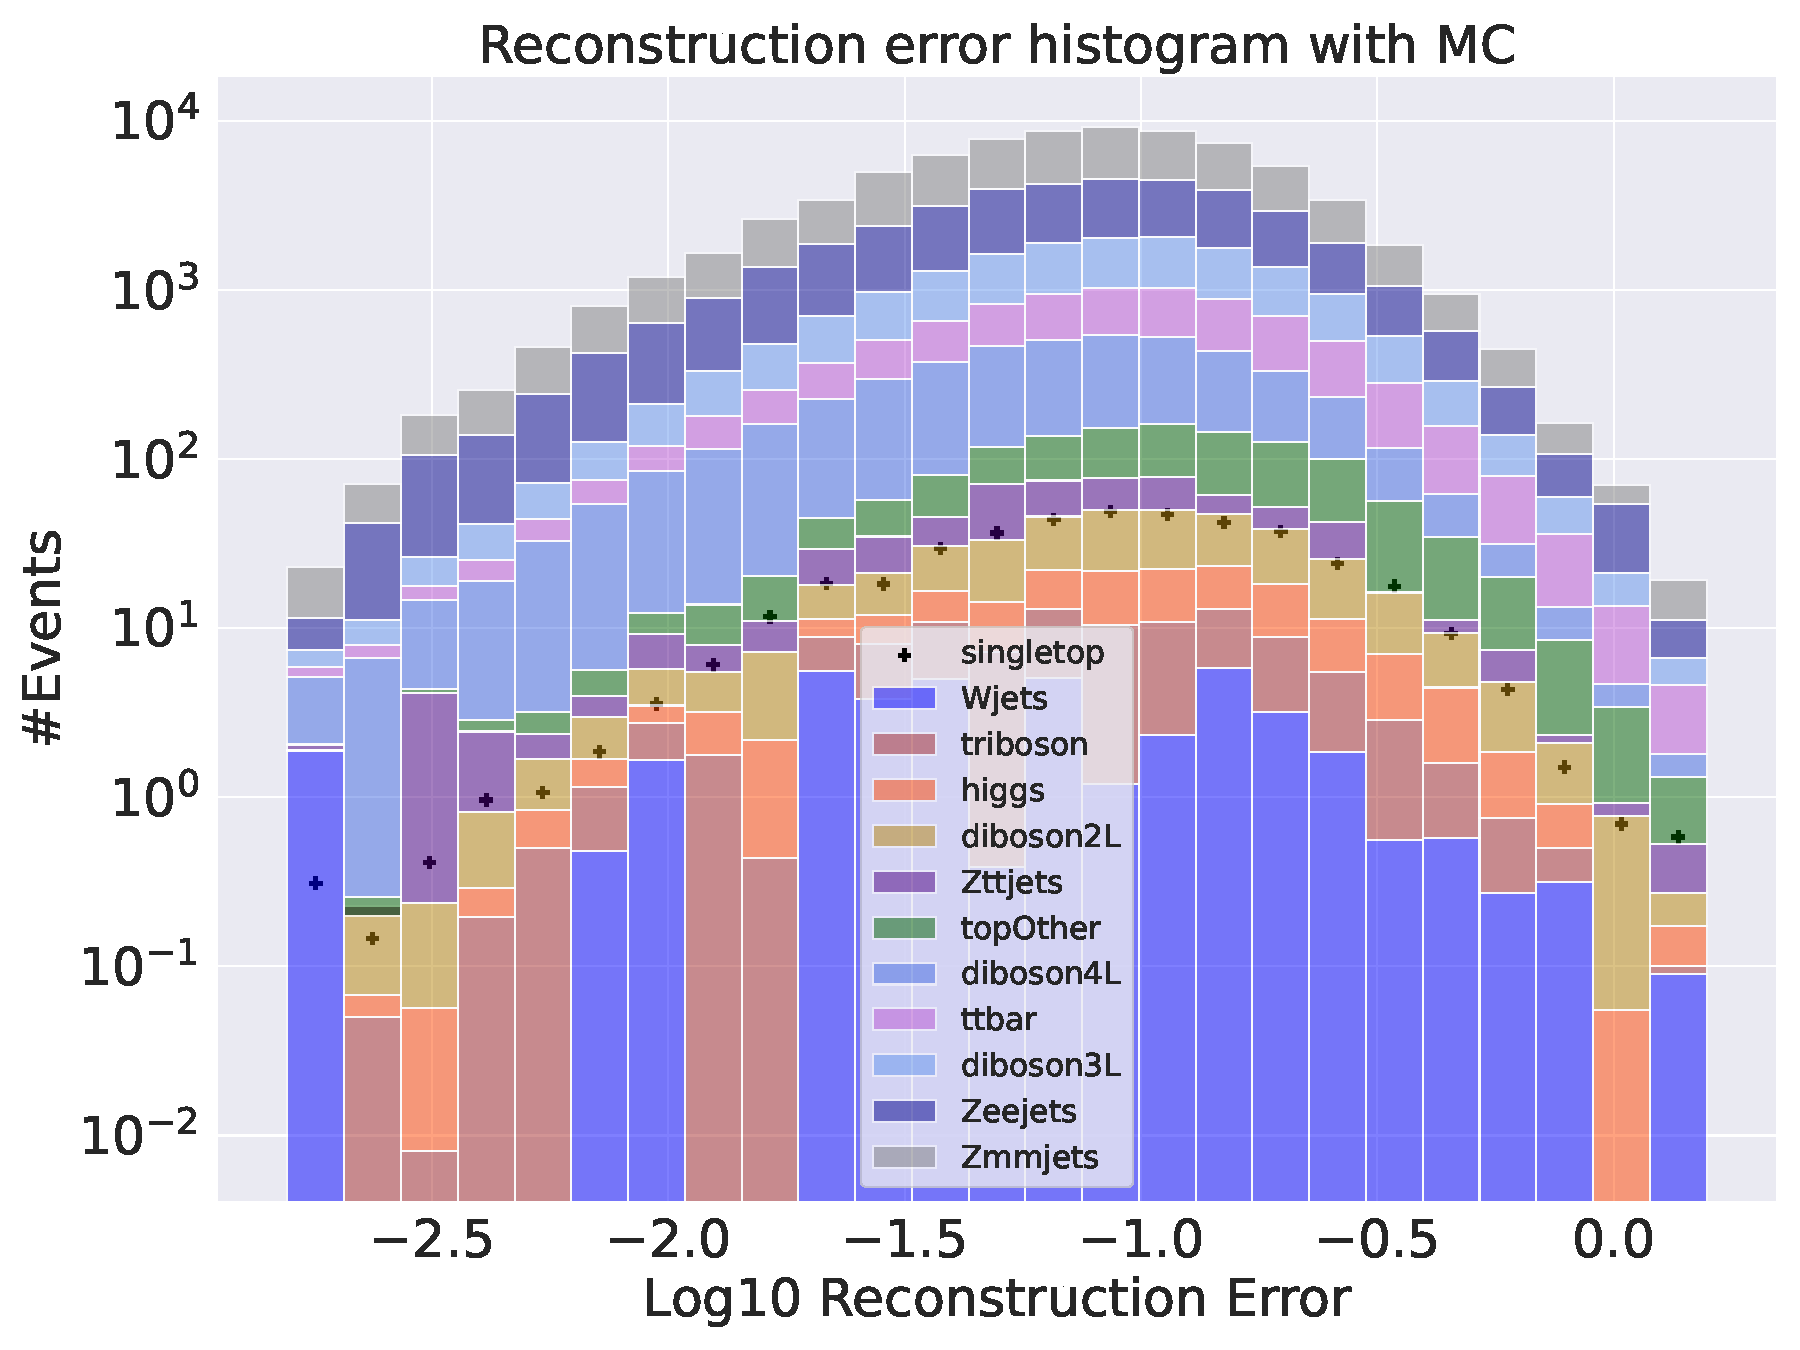
\includegraphics[width=\textwidth]{Figures/VAE_testing/small/b_data_recon_big_rm3_feats_sig_singletop.pdf}
        \caption{Reconstruction error on validation SM MC from the small variational Autoencoder. Here the singletop channel has been removed from training and 
        is used as signal. No significant difference in distributions are found. }
        \label{fig:vae_small_singletop}
    \end{subfigure}
    \hfill
    \begin{subfigure}{.45\textwidth}
        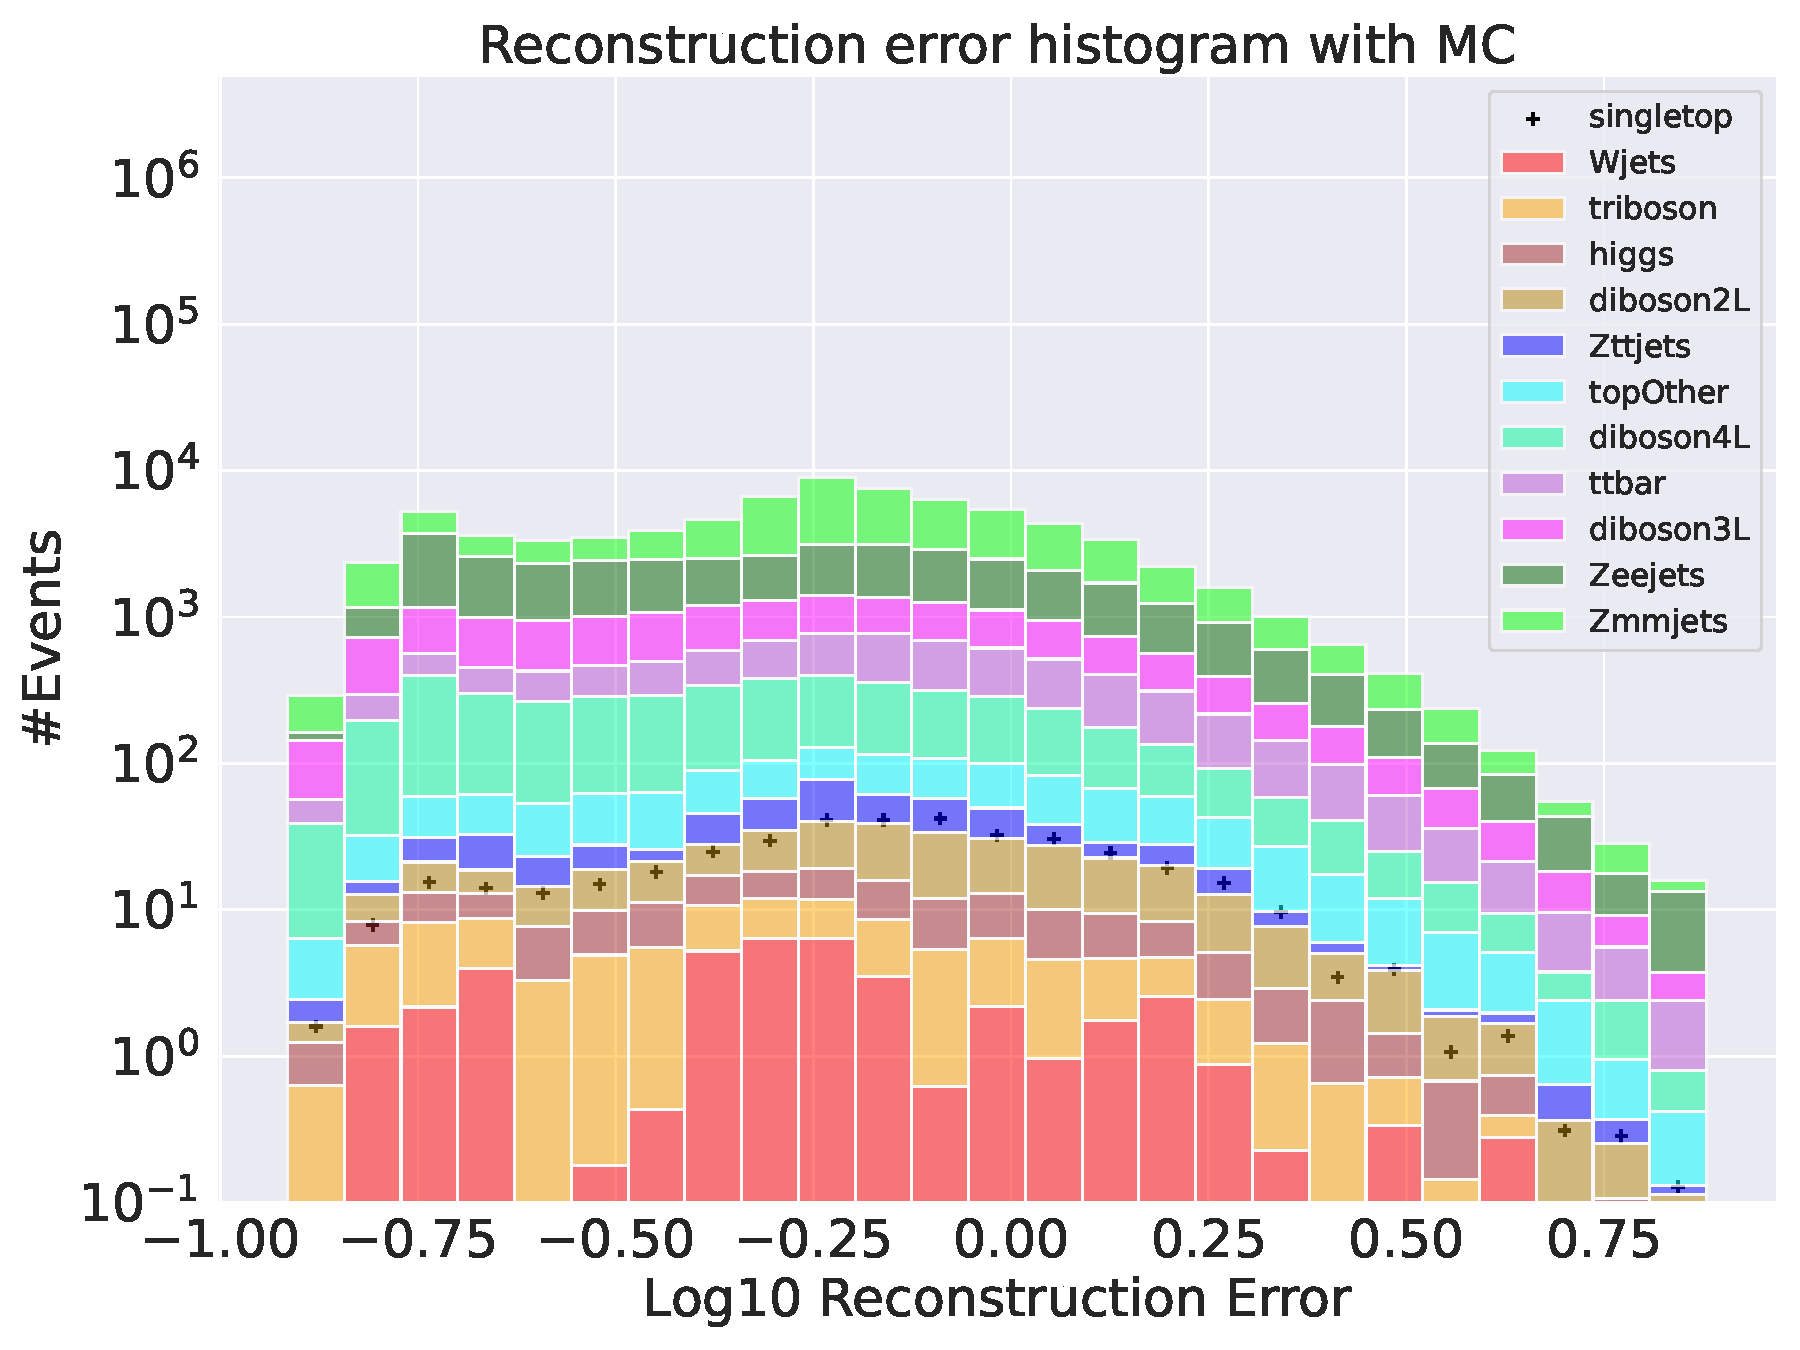
\includegraphics[width=\textwidth]{Figures/VAE_testing/big/b_data_recon_big_rm3_feats_sig_singletop.pdf}
        \caption{Reconstruction error on validation SM MC from the big variational Autoencoder. Here the singletop channel has been removed from training and 
        is used as signal. No significant difference in distributions are found. }
        \label{fig:vae_big_singletop}
    \end{subfigure}
    \hfill 
    \label{fig:vae_big_channel_2}
\end{figure}

\begin{figure}[h!]
    \centering
    \begin{subfigure}{.45\textwidth}
        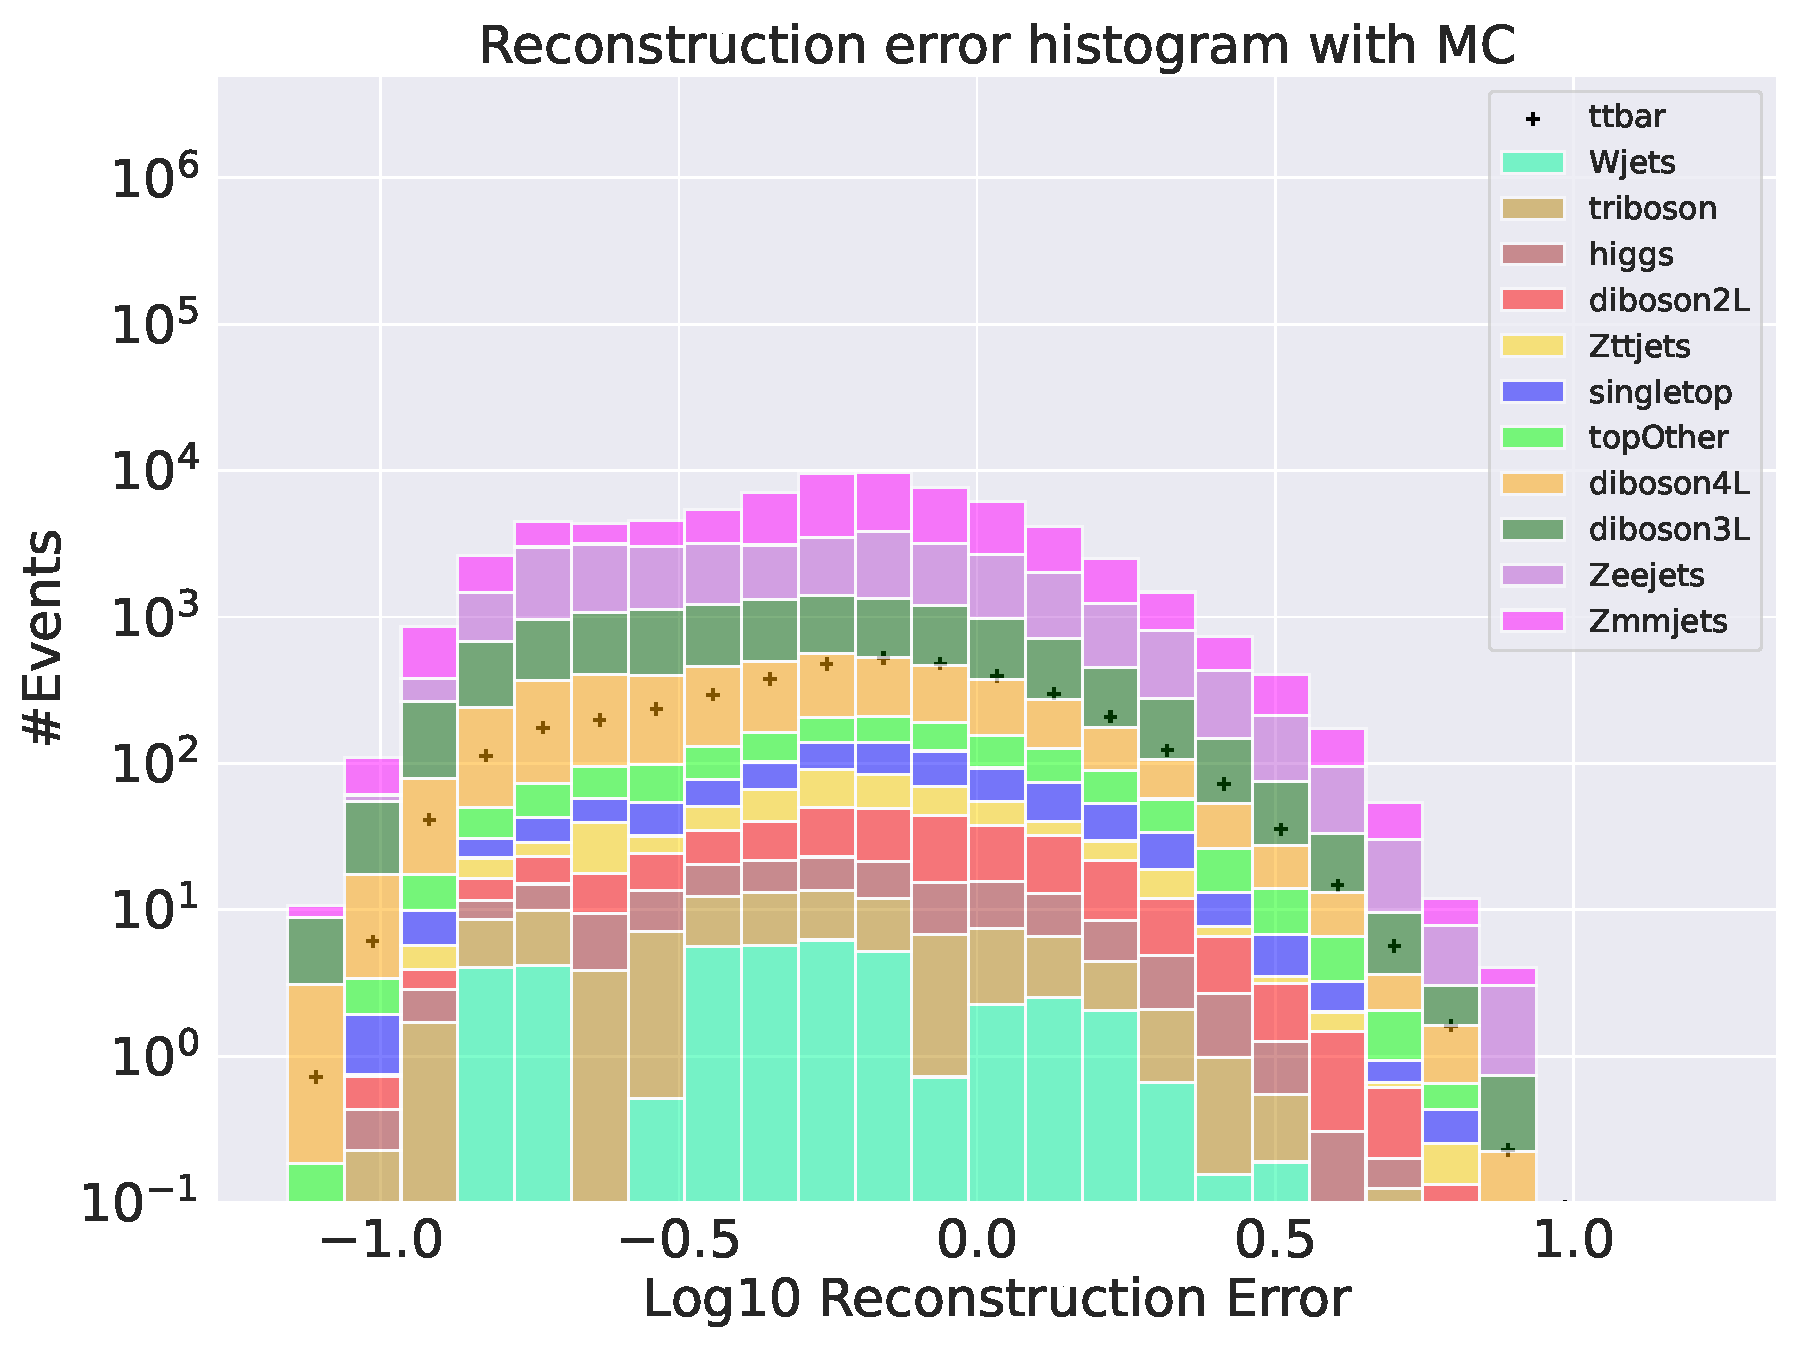
\includegraphics[width=\textwidth]{Figures/VAE_testing/small/b_data_recon_big_rm3_feats_sig_ttbar.pdf}
        \caption{Reconstruction error on validation SM MC from the small variational Autoencoder. Here the ttbar channel has been removed from training and 
        is used as signal. No significant difference in distributions are found. }
        \label{fig:vae_small_ttbar}
    \end{subfigure}
    \hfill 
    \begin{subfigure}{.45\textwidth}
        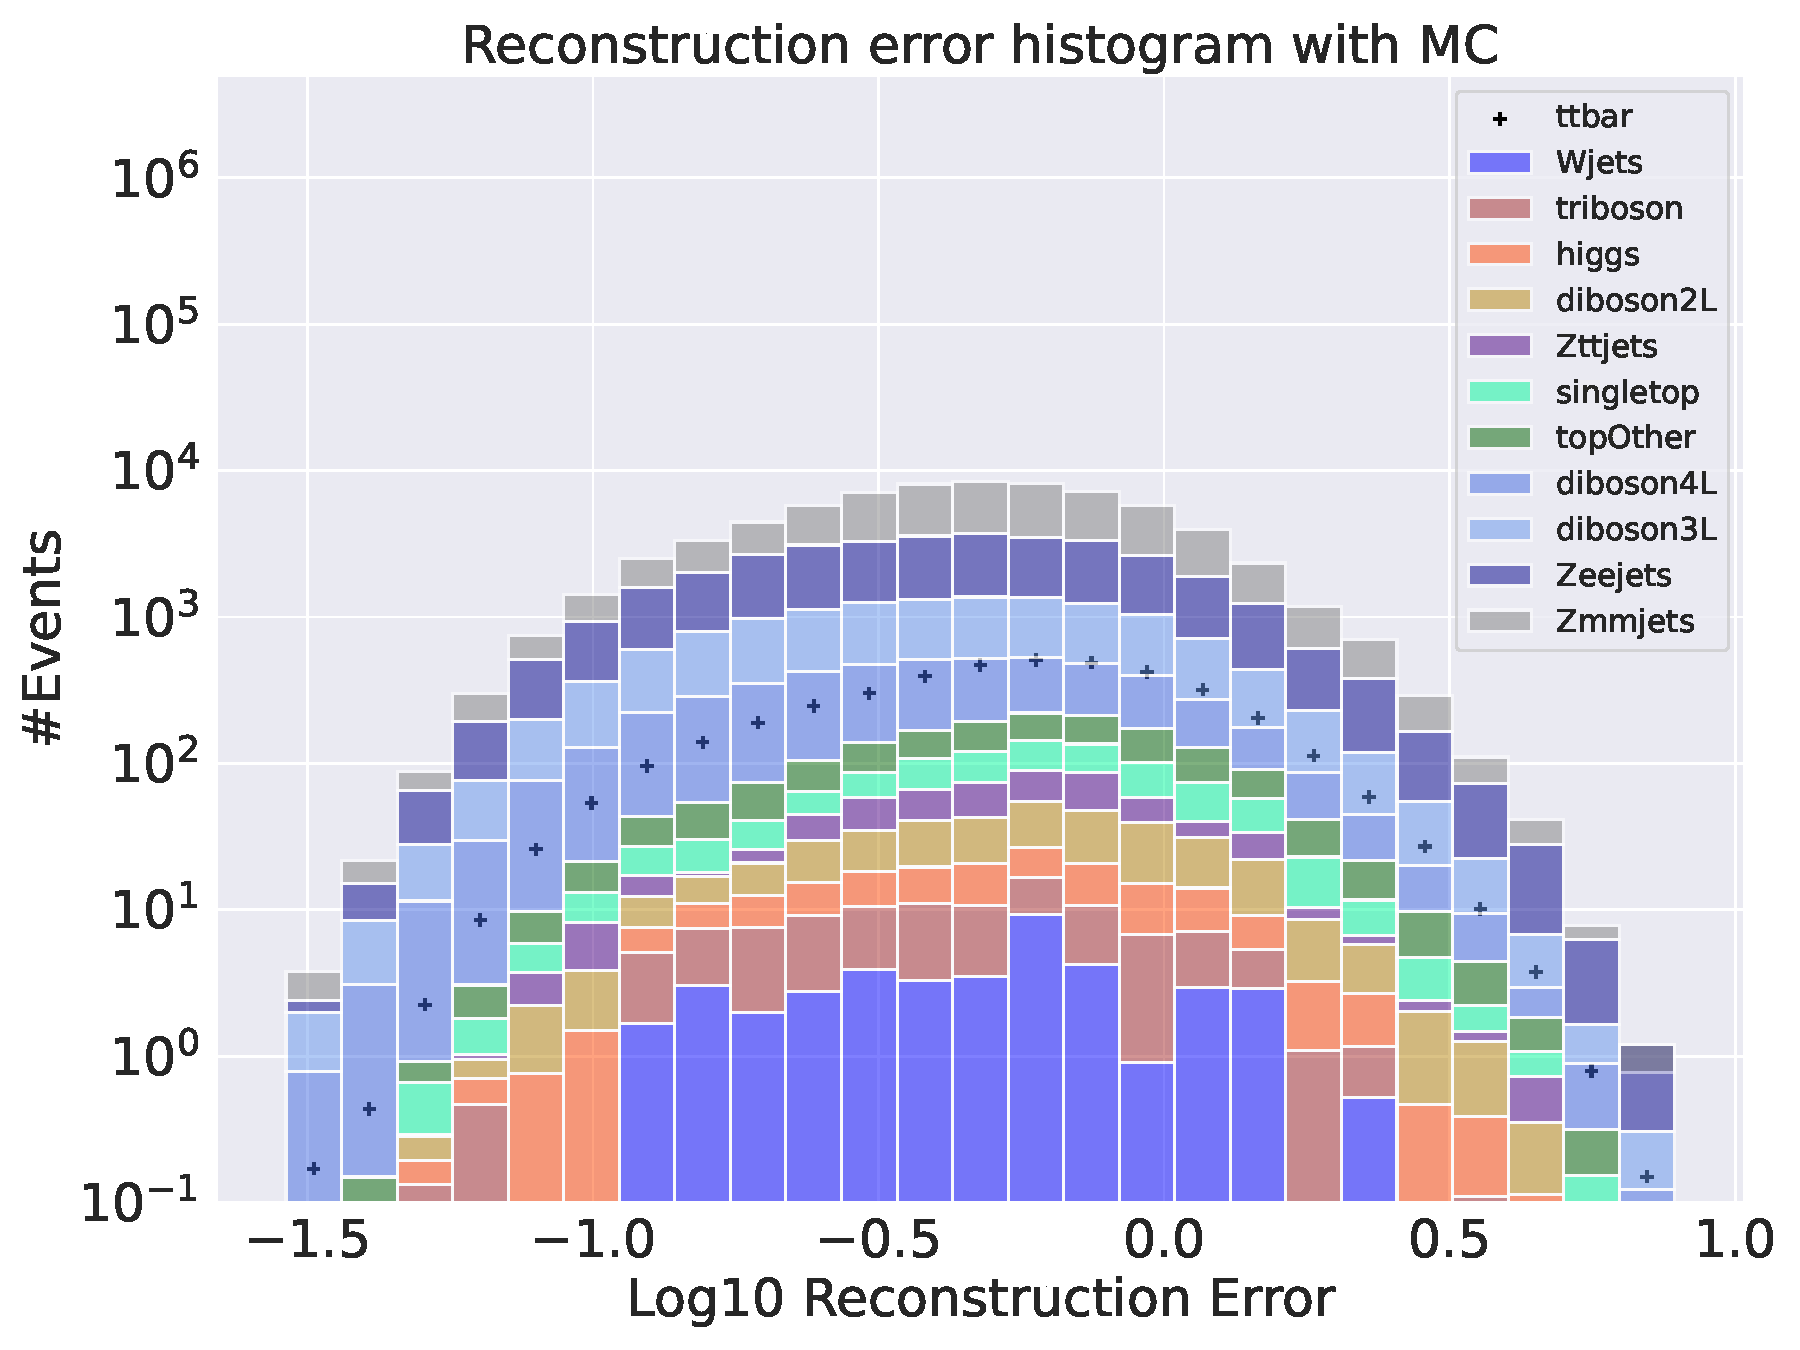
\includegraphics[width=\textwidth]{Figures/VAE_testing/big/b_data_recon_big_rm3_feats_sig_ttbar.pdf}
        \caption{Reconstruction error on validation SM MC from the big variational Autoencoder. Here the ttbar channel has been removed from training and 
        is used as signal. No significant difference in distributions are found. }
        \label{fig:vae_big_ttbar}
    \end{subfigure}
    \hfill 
    \label{fig:vae_big_channel_3}
\end{figure}